\documentclass{article}

% Language setting
% Replace `english' with e.g. `spanish' to change the document language
\usepackage[english]{babel}
\usepackage{subcaption}
% Set page size and margins
% Replace `letterpaper' with `a4paper' for UK/EU standard size
\usepackage[letterpaper,top=2cm,bottom=2cm,left=3cm,right=3cm,marginparwidth=1.75cm]{geometry}

% Useful packages
\usepackage{amsmath}
\usepackage{graphicx}
\usepackage[colorlinks=true, allcolors=blue]{hyperref}

\title{Image Interpolation with Diffusion Models}
\author{Yankai Mao(ym3121)}

\begin{document}
\maketitle


\section{Overview}
Image interpolation with diffusion models has rapidly evolved from simple latent blending to structured, geometry- and probability-aware path generation. Early work such as \textit{Interpolating between Images with Diffusion Models}~\cite{wang2023interpolating} introduced a training-free pipeline that combines latent, noise, and text interpolation, but suffers from semantic instability and artifacts. Subsequent methods improve interpolation quality by introducing additional structure: \textit{DiffMorpher}~\cite{zhang2023diffmorpher} interpolates LoRA parameters, noise, and attention features to achieve smoother and more consistent morphing, at the cost of per-image optimization; \textit{DreamMover}~\cite{xing2024dreammover} extends interpolation to large-motion scenarios by incorporating diffusion priors with flow estimation and attention fusion; and attention-based approaches such as \textit{AID: Attention Interpolation of Text-to-Image Diffusion}~\cite{li2024aid} improve controllability in conditional generation. More recent work, \textit{Probability Density Geodesics in Image Diffusion Latent Space}~\cite{chen2025geodesic}, reframes interpolation as finding paths along high-probability regions of the diffusion latent space, addressing the fundamental issue that linear interpolation often traverses unrealistic low-density regions. 

Overall, existing methods can be categorized into latent-space interpolation, noise/trajectory interpolation, parameter (e.g., LoRA)-space interpolation, and attention-based interpolation, each offering different trade-offs in smoothness, semantic consistency, controllability, and computational cost. 

Despite significant progress, key challenges remain, including degeneration, hallucination, identity drift, and the lack of reliable evaluation metrics, motivating future research toward geometry-aware, flow-based, and unified interpolation frameworks.

In this project, we reproduce \textit{Interpolating between
  Images with Diffusion Models}~\cite{wang2023interpolating},
  implementing the core interpolation pipeline with modified
  conditioning strategies and analyzing the method's capabilities
  and constraints.




% Image interpolation with diffusion models has developed from simple latent interpolation to more structured approaches. Early work such as \textit{Interpolating between Images with Diffusion Models}~\cite{wang2023interpolating} uses latent, noise, and text interpolation in a training-free way, but often produces unstable results. Later methods improve quality by adding more control: \textit{DiffMorpher}~\cite{zhang2023diffmorpher} interpolates LoRA parameters and attention features for smoother transitions, while \textit{DreamMover}~\cite{xing2024dreammover} focuses on large motion using flow and attention fusion. Attention-based methods like \textit{AID}~\cite{li2024aid} improve controllability, and recent work such as \textit{Probability Density Geodesics}~\cite{chen2025geodesic} shows that better interpolation paths can be found by staying in high-probability regions instead of using simple linear interpolation. Overall, methods can be grouped into latent-space, noise/trajectory, parameter-space, and attention-based interpolation, each with trade-offs in quality and efficiency. However, problems like artifacts, identity drift, and evaluation are still not fully solved.


\section{Problem Formulation}

Given two input images $x_0$ and $x_1$, the goal of image interpolation is to generate a sequence of intermediate images $\{x_\alpha\}_{\alpha \in [0,1]}$ such that:
\begin{itemize}
    \item $x_{\alpha=0} = x_0$ and $x_{\alpha=1} = x_1$,
    \item the transition is smooth with respect to $\alpha$,
    \item intermediate images remain realistic and semantically consistent.
\end{itemize}

In diffusion-based methods, this is typically achieved by mapping images into a latent space and defining an interpolation path:
\[
z_\alpha = (1 - \alpha) z_0 + \alpha z_1,
\]
where $z_0$ and $z_1$ are latent representations of $x_0$ and $x_1$. The interpolated latent $z_\alpha$ is then decoded through the diffusion model to obtain $x_\alpha$.


\section{Method}

\begin{figure}
\centering
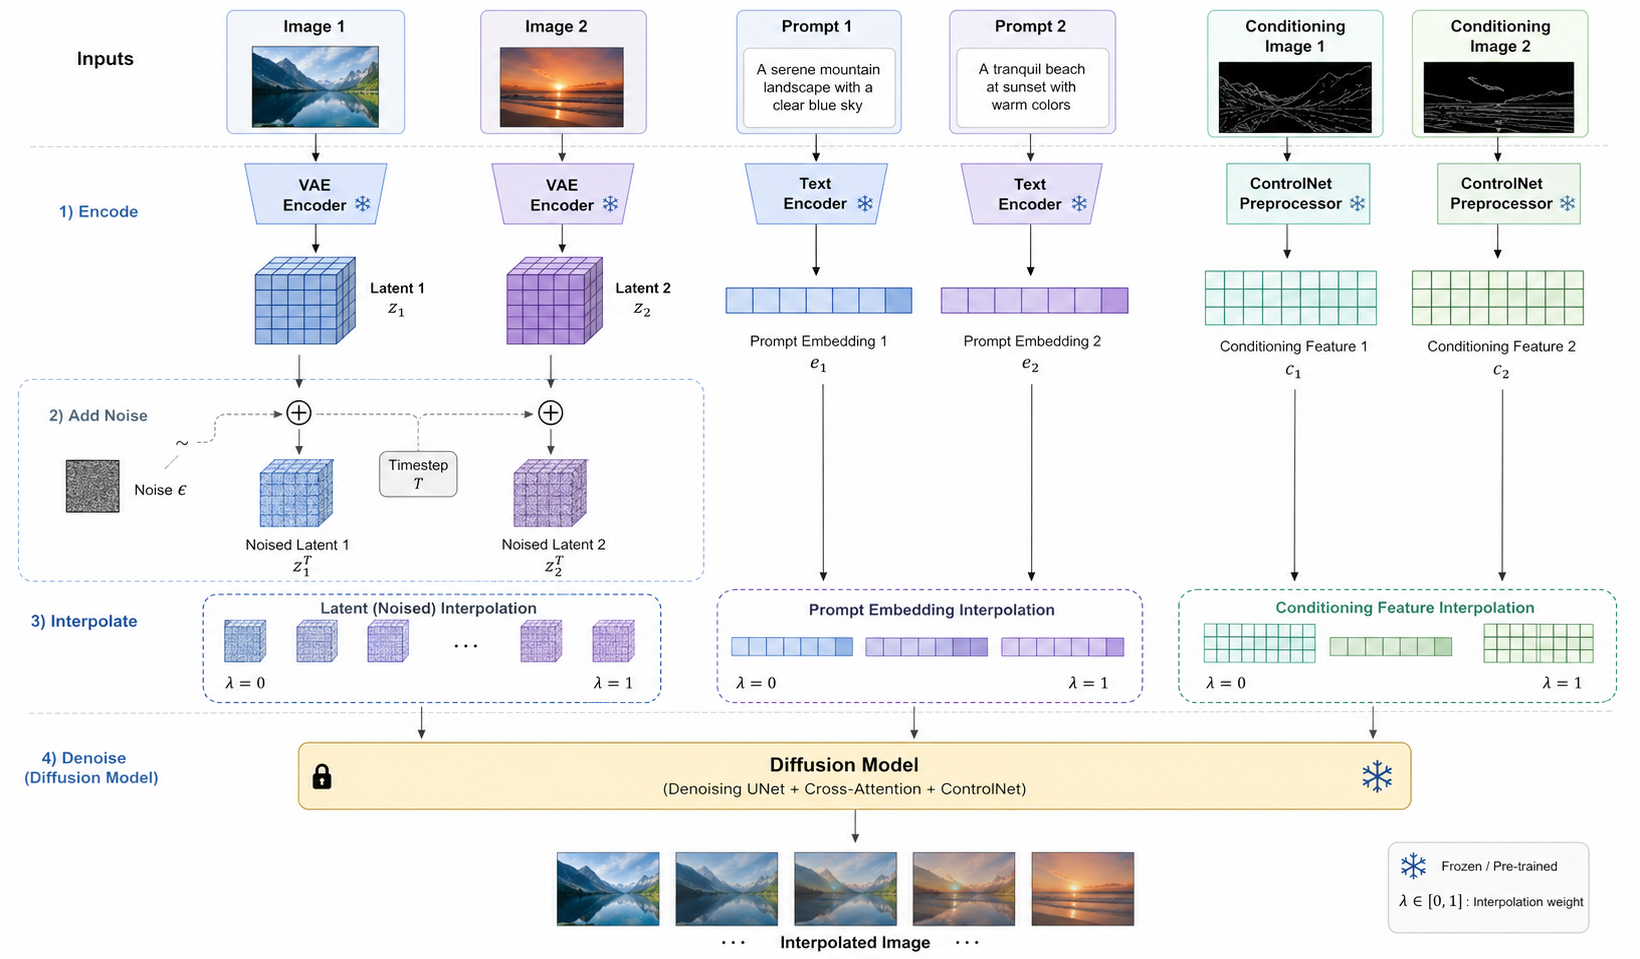
\includegraphics[width=0.9\linewidth]{interpolation_process.png}
\caption{\label{fig:interpolation}The pipeline for each interpolation process.}
\end{figure}

\subsection{Iterative Interpolation}
Given $N$ interpolation steps, we take two input images denoted as
$I_0$ and $I_N$. In the first step, we interpolate between $I_0$
and $I_N$ to generate the midpoint $I_{N/2}$. Next, we recursively
interpolate between consecutive pairs: $I_0$ and $I_{N/2}$ yield
$I_{N/4}$, while $I_{N/2}$ and $I_N$ yield $I_{3N/4}$. This       
process continues iteratively until we obtain the complete
sequence $I_0, I_1, \ldots, I_N$. At each step, we generate
multiple candidate frames and select the best one either manually
or via CLIP scoring~\cite{radford2021clip}.


\subsection{Interpolation Mechanics}

As shown in Figure~\ref{fig:interpolation}, our approach feeds
three interpolated components into Stable Diffusion 1.5~\cite{rombach2022ldm, sd15}. We first
encode both input images through the VAE encoder to obtain latent
representations $z_1$ and $z_2$, then add identical noise to both.
The noise level $t$ is adaptive: frames closer to the endpoints
use smaller $t$ values to minimize variation. We interpolate the
noised latent tensors linearly to obtain the intermediate latent
representation. 


For text conditioning, we explore two approaches: (1) optimizing a
single prompt embedding via textual inversion to minimize the
loss $\mathcal{L}(c_\text{prompt}) = \| \epsilon_\theta(z_t,
c_\text{prompt}) - \epsilon \|^2$, where $z_t$ denotes the noised
latent and $\epsilon$ is the ground-truth noise; (2) directly
providing two manual prompts describing each image, then
interpolating their CLIP embeddings.


For spatial conditioning, we extract either edge maps or pose
keypoints using ControlNet auxiliary detector. For non-photorealistic
images, we first apply image-to-image translation with a
photorealistic style guidance prompt before extracting control
features. These conditioning features are then linearly
interpolated between the two inputs.

\section{Results \& Analysis}
  We conduct experiments on an A100 GPU using 200 DDIM steps for    
  improved quality. Generating a complete 32-frame interpolation
  sequence requires approximately 30 minutes.                       
                                                            
  When input images have similar structural layouts (i.e., similar
  edge maps), the method generates plausible transitions as
  demonstrated in Figure~\ref{fig:inter_results}.

  However, the results exhibit high sensitivity to spatial
  conditioning. Without ControlNet guidance, interpolated frames
  become unstable. When using edge conditioning—the most common
  configuration—the interpolated edge maps contain overlapping edges
   from both inputs, and these overlapping regions produce visual
  artifacts in the generated frames. For image pairs with large
  semantic, stylistic, or structural gaps (e.g., photorealistic to
  anime, vastly different edge maps), the method struggles to
  produce smooth transitions, as shown in Figure~\ref{fig:failure}.

  Regarding textual inversion, we observe that the loss fluctuates
  periodically without converging, even when increasing optimization
   steps from 200 to 1000. When images differ semantically, the
  shared initial prompt often poorly describes one input. To address
   this, we experimented with providing two distinct prompts
  describing each image separately. This approach yields comparable
  performance with improved stability.
\begin{figure}[t]
\centering

% Row 1
\begin{subfigure}{0.22\linewidth}
    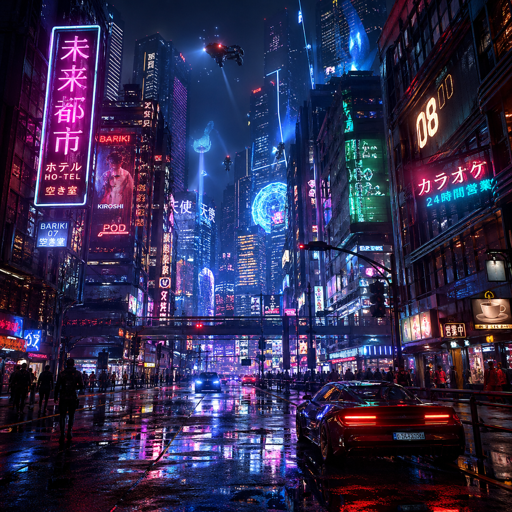
\includegraphics[width=\linewidth]{results/city0.png}
\end{subfigure}
\begin{subfigure}{0.22\linewidth}
    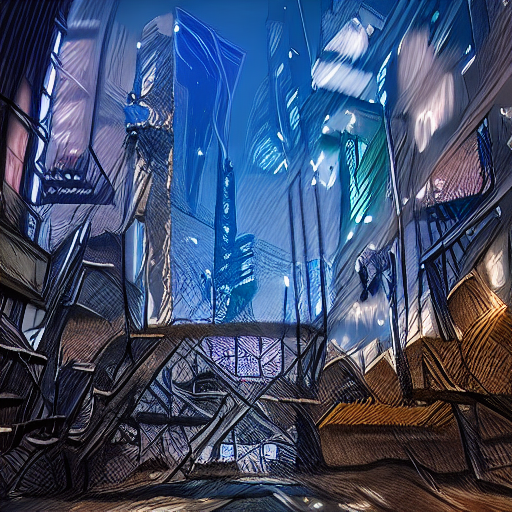
\includegraphics[width=\linewidth]{results/city1.png}
\end{subfigure}
\begin{subfigure}{0.22\linewidth}
    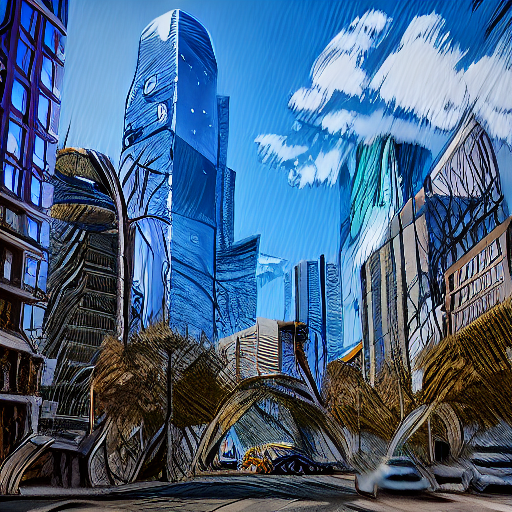
\includegraphics[width=\linewidth]{results/city2.png}
\end{subfigure}
\begin{subfigure}{0.22\linewidth}
    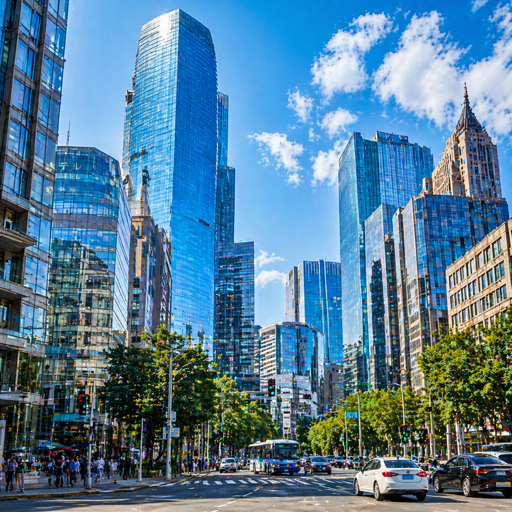
\includegraphics[width=\linewidth]{results/city3.png}
\end{subfigure}

\vspace{0.5em}

% Row 2
\begin{subfigure}{0.22\linewidth}
    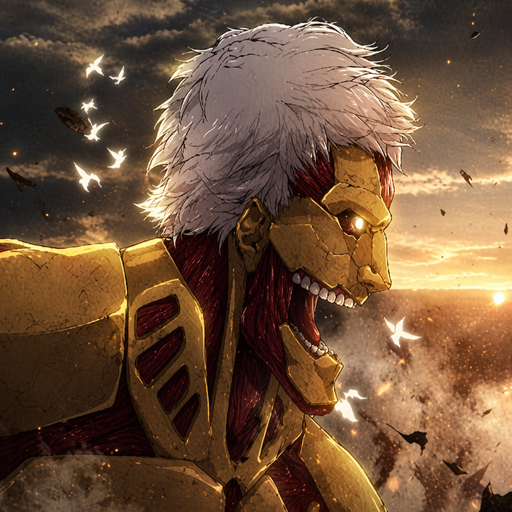
\includegraphics[width=\linewidth]{results/titan0.png}
\end{subfigure}
\begin{subfigure}{0.22\linewidth}
    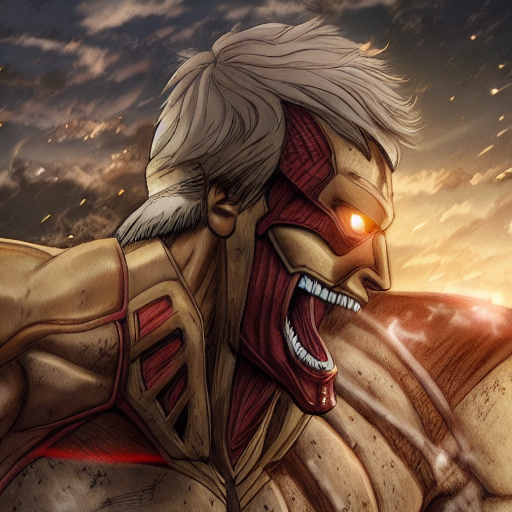
\includegraphics[width=\linewidth]{results/titan1.png}
\end{subfigure}
\begin{subfigure}{0.22\linewidth}
    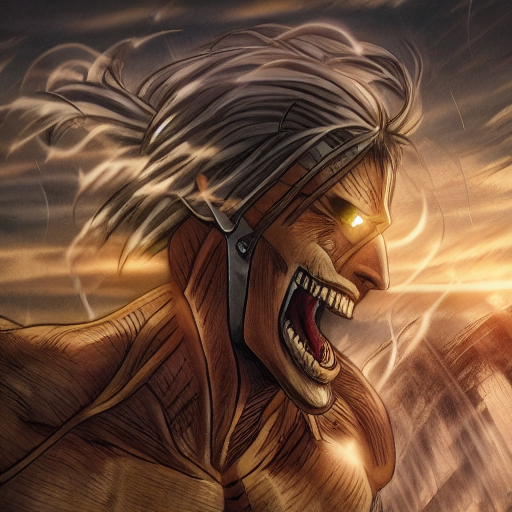
\includegraphics[width=\linewidth]{results/titan2.png}
\end{subfigure}
\begin{subfigure}{0.22\linewidth}
    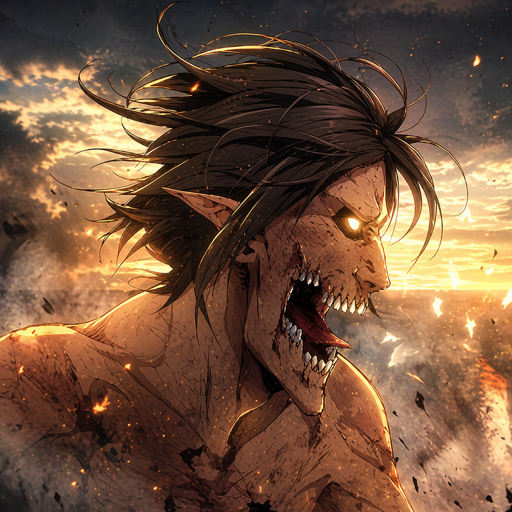
\includegraphics[width=\linewidth]{results/titan3.png}
\end{subfigure}

\caption{Interpolation results.}
\label{fig:inter_results}
\end{figure}


\begin{figure}[t]
\centering

% Row 1
\begin{subfigure}{0.17\linewidth}
    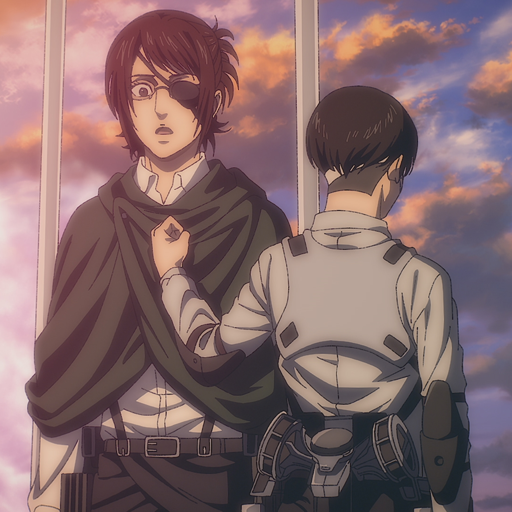
\includegraphics[width=\linewidth]{results/failure/two_men0.png}
\end{subfigure}
\begin{subfigure}{0.17\linewidth}
    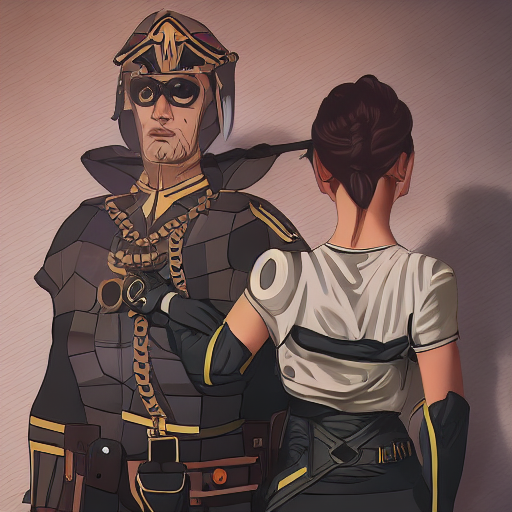
\includegraphics[width=\linewidth]{results/failure/two_men1.png}
\end{subfigure}
\begin{subfigure}{0.17\linewidth}
    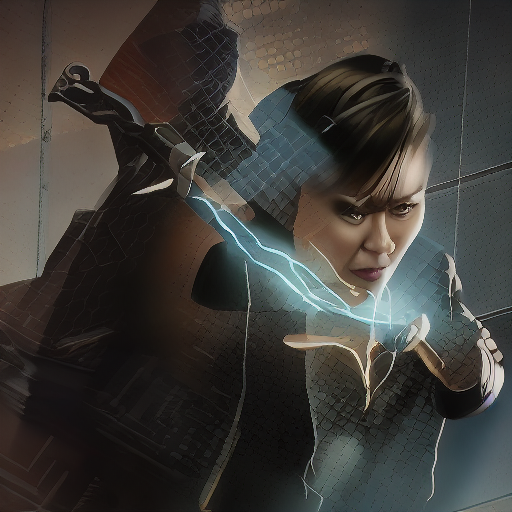
\includegraphics[width=\linewidth]{results/failure/two_men2.png}
\end{subfigure}
\begin{subfigure}{0.17\linewidth}
    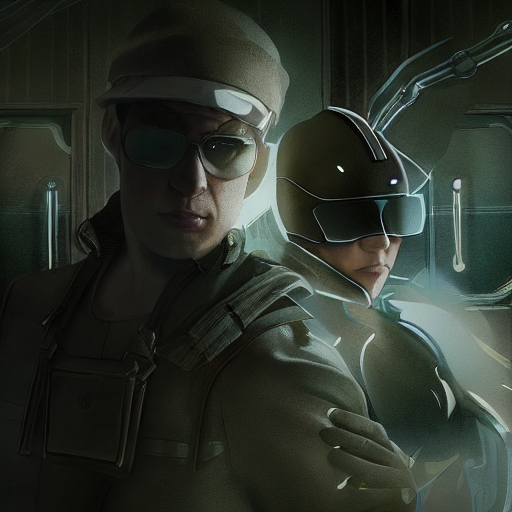
\includegraphics[width=\linewidth]{results/failure/two_men3.png}
\end{subfigure}
\begin{subfigure}{0.17\linewidth}
    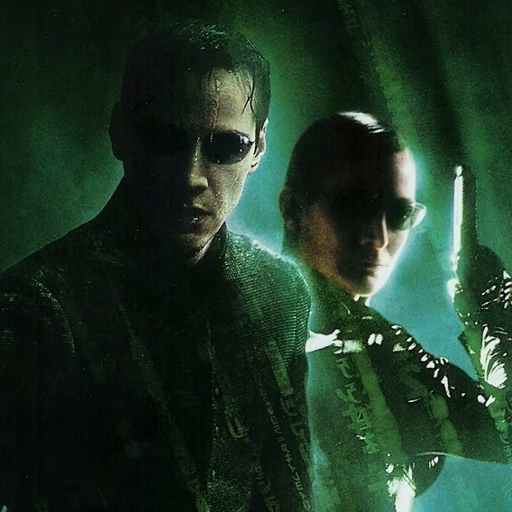
\includegraphics[width=\linewidth]{results/failure/two_men4.png}
\end{subfigure}

\vspace{0.5em}

% Row 2
\begin{subfigure}{0.17\linewidth}
    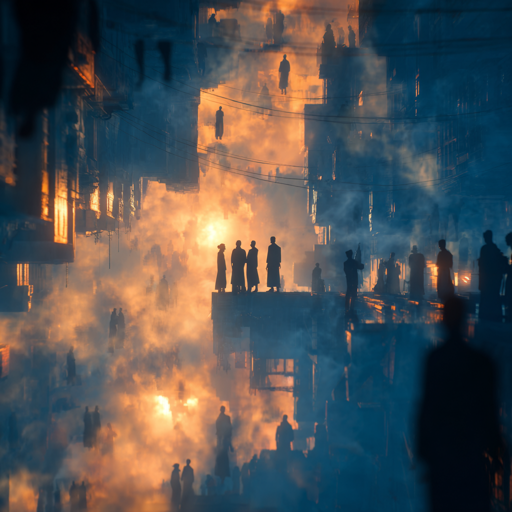
\includegraphics[width=\linewidth]{results/failure/dream0.png}
\end{subfigure}
\begin{subfigure}{0.17\linewidth}
    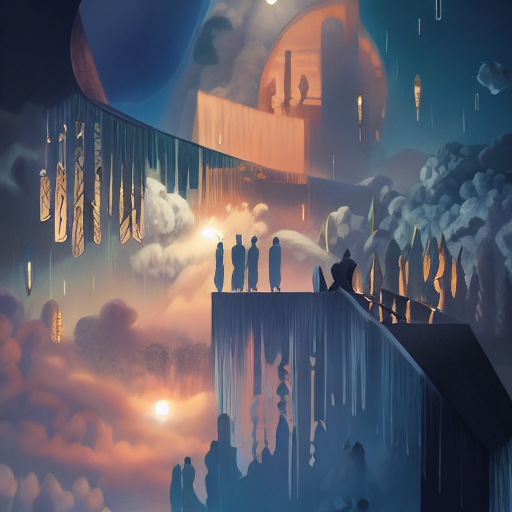
\includegraphics[width=\linewidth]{results/failure/dream1.png}
\end{subfigure}
\begin{subfigure}{0.17\linewidth}
    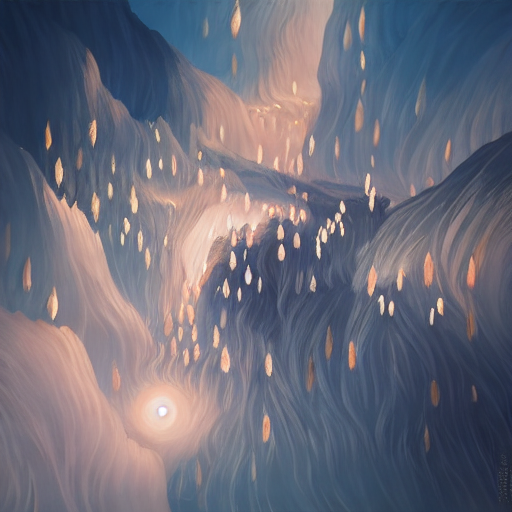
\includegraphics[width=\linewidth]{results/failure/dream2.png}
\end{subfigure}
\begin{subfigure}{0.17\linewidth}
    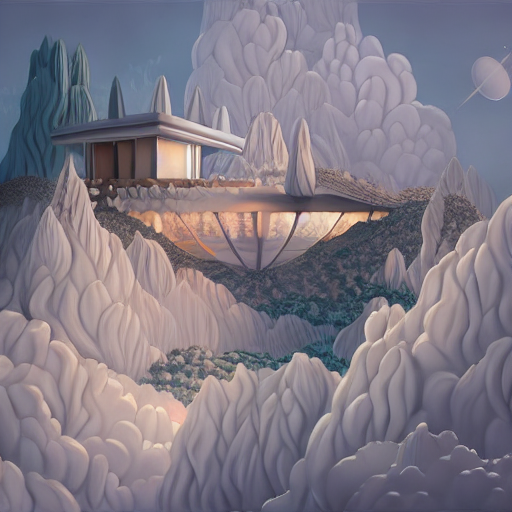
\includegraphics[width=\linewidth]{results/failure/dream3.png}
\end{subfigure}
\begin{subfigure}{0.17\linewidth}
    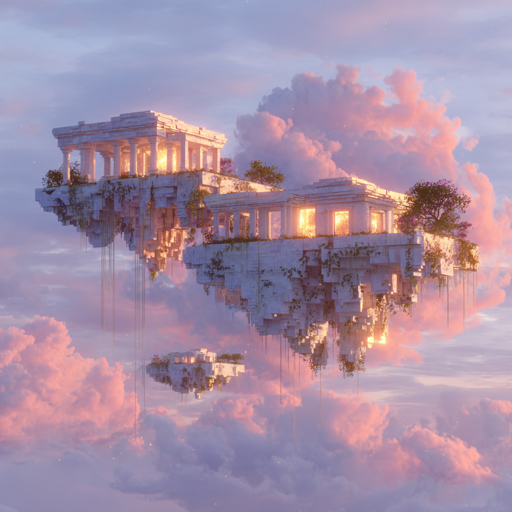
\includegraphics[width=\linewidth]{results/failure/dream4.png}
\end{subfigure}

\caption{Failure cases.}
\label{fig:failure}
\end{figure}



\section{Future Work}

Future work could extend this analysis with quantitative
  evaluation metrics to complement our qualitative observations.

  
  Additionally, it would be interesting to explore whether a        
  systematic taxonomy of image transitions might reveal distinct
  interpolation behaviors. Such a taxonomy could categorize         
  transitions by their dominant characteristics—temporal continuity
  (video-like sequences), stylistic shifts (photorealistic to
  artistic), semantic changes (cross-category transformations),
  structural variations (pose and layout), and identity transitions
  (same category, different instances). If each transition type
  exhibits specific features or failure patterns, this could provide
   insights into the fundamental characteristics of diffusion-based
  interpolation and potentially inform the development of
  specialized or adaptive approaches for different scenarios.

\begin{thebibliography}{9}

\bibitem{wang2023interpolating}
T. Wang and P. Golland. 
\newblock Interpolating between Images with Diffusion Models.
\newblock \textit{ICML Workshop}, 2023. 
\newblock \url{https://arxiv.org/abs/2307.12560}

\bibitem{zhang2023diffmorpher}
K. Zhang et al.
\newblock DiffMorpher: Unleashing the Capability of Diffusion Models for Image Morphing.
\newblock \textit{CVPR}, 2024.
\newblock \url{https://arxiv.org/abs/2312.07409}

\bibitem{xing2024dreammover}
J. Xing et al.
\newblock DreamMover: Leveraging the Prior of Diffusion Models for Image Interpolation with Large Motion.
\newblock \textit{ECCV}, 2024.
\newblock \url{https://arxiv.org/abs/2409.09605}

\bibitem{li2024aid}
X. Li et al.
\newblock AID: Attention Interpolation of Text-to-Image Diffusion.
\newblock \textit{NeurIPS}, 2024.
\newblock \url{https://arxiv.org/abs/2403.17924}

\bibitem{chen2025geodesic}
Y. Chen et al.
\newblock Probability Density Geodesics in Image Diffusion Latent Space.
\newblock \textit{CVPR}, 2025.
\newblock \url{https://arxiv.org/abs/2504.06675}

\bibitem{rombach2022ldm}
R. Rombach, A. Blattmann, D. Lorenz, P. Esser, and B. Ommer. 
\newblock High-Resolution Image Synthesis with Latent Diffusion Models. 
\newblock \textit{CVPR}, 2022. 
\newblock \url{https://arxiv.org/abs/2112.10752}

\bibitem{sd15}
Stability AI. 
\newblock Stable Diffusion v1.5. 
\newblock 2022. 
\newblock \url{https://github.com/CompVis/stable-diffusion}

\bibitem{radford2021clip}
A. Radford et al.
\newblock Learning Transferable Visual Models From Natural Language Supervision.
\newblock In \textit{ICML}, 2021.
\newblock \url{https://arxiv.org/abs/2103.00020}

\end{thebibliography}

\end{document}
